\thispagestyle{plain}
\chapter{Framework}
This chapter introduces the framework that was implemented to generate workloads, partition data and eventually benchmark a custom index that uses the partitioning. Note that the terms partitions and segments will be used interchangeably in the following.
\begin{figure}[H]
    \centering
    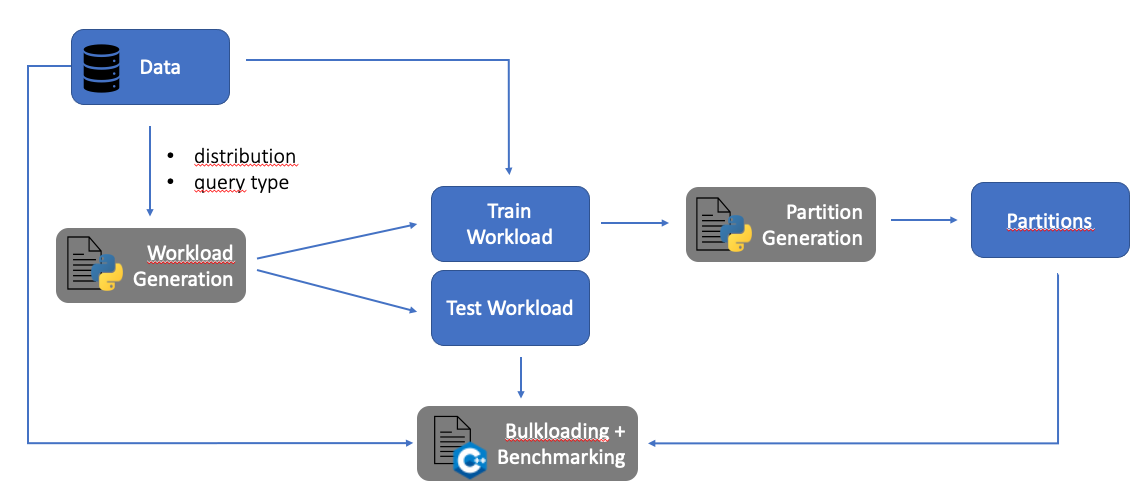
\includegraphics[width=\textwidth]{figures/pipeline.png}
    \caption{Framework Overview}
    \label{fig:framework}
\end{figure}

\section{Overview}
As we can see in Figure \ref{fig:framework}, the origin of all processes is the underlying data that we want to index. Using a python script, we can specify properties like the distribution and type of queries (point, range) that should be generated to access the data through the index. The queries generated by this step are divided into a train and test workload and saved to files for later use in the C++ benchmarking.

Given the train workload, the partitioning algorithms that are described in Sections \ref{sec:frequency} and \ref{sec:purity} can analyze the corresponding properties of the workload and will produce a partition of the underlying data. The resulting elements are saved to a file with additional information that can be used for the index construction. This information as of now indicates the relative frequency of a segment compared to the others and whether the segment mostly received point queries.
With this partition, the index is bulkloaded from the data where each element of the partition corresponds to an individual leaf node. The additional information is used to modify the structure and physical specialization of our index. For example, if only point queries access a segment, it could be beneficial to manage data access through a hash table instead of a normal B-tree leaf. The next step is to execute the test workload on the index and compare it to other state-of-the-art indexes that were introduced in Section \ref{sec:related_work}, namely a B$^+$-tree, an Adaptive Radix Tree (ART) and a Piecewise Geometric Model index (PGM).

\section{Workload Generation} \label{sec:wklgeneration}
The ultimate goal of this work is to generate good partitions for the index construction like it was mentioned in Section \ref{bg:hybrid}. The inputs to the partitioning algorithms are therefore a dataset and a workload sample which we know is representative of the expected workload. However, for the purpose of evaluating and testing the algorithms and modifications later used, we were in need of a flexible way to generate workload data, especially since it proved hard to find available real-world workload data. Although we do not have real-word workload data, we used also used our synthetic workload generation on real-world datasets, in the hope that we get representative results. The workload generation is done in a Python script specifying a series of \verb|Region| objects. The idea is, that we have a basic repertoire of distributions (like uniform, zipfian, ...) that we append or overlap to create many different and more complex workloads. The \verb|Region| objects contain the following information:

\begin{itemize}
    \item \verb|index|: Whether the generation happens index-based or domain-based. Index-based means that we draw valid indices according to a distribution and then resolve the data values at these indices, domain-based means that we draw from the domain of the data, i.e.~we can draw values that fall inside the domain, but are not present in the data itself. This cannot happen for index-based generation.
    \item \verb|min, max|: The Minimal and maximal values that indicate the region boundaries. These represent either the minimum and maximum index in the dataset (index-based) or the range of values from the data domain from which values can be generated (domain-based).
    \item \verb|qtype|: The query type that should be generated in this region, e.g.~point or range queries
    \item \verb|num|: The number of queries in this region
    \item \verb|distribution|: The distribution underlying the generated queries in the region, e.g.~normal, uniform, ...
\end{itemize}

This gives us a very flexible way to generate arbitrary workloads. Note that while a partition generated for the index construction later satisfies that the elements are mutually disjoint, the \verb|Region| objects used for workload generation do not need to be disjoint. This only means that we can overlap the boundaries of the objects to generate even more flexible workloads. In fact, it is the only way to generate regions of the data that are accessed through multiple types of queries, e.g.~through both point and range queries. 

After the queries are generated, we randomly sample a given fraction of them and remove these from the original queries. Similar to Machine Learning methods, we only use one of the resulting two sets to create our partitions (training), the second set is later used for evaluation (testing) and immediately saved to a file. This ensures that we do not just design partitions that are optimal for the training queries. Instead, the partitions should be suitable for the underlying population of which train and test workload are only samples.

\section{Partitioning algorithms}
The next step in the framework is to use the train workload to find partitions in the data. There are many properties that one could look at when analyzing query workloads, but inspired by the works in Section \ref{sec:related_work}, we decided to focus on two properties and look at how we could use these to partition the data and create segments: Frequency and Purity.

\subsection{Partitioning by Frequency} \label{sec:frequency}
The first algorithm analyzes the frequency of query accesses for each key in our dataset. The motivation behind using the frequency as a partition property is that, hopefully, we can benefit from caching effects during execution of the test workload. We would hope that the path to highly frequent segments remains in cache so that subsequent queries can retrieve the location of the corresponding keys faster. On the other hand, the path to segments that are almost never touched should not be present in cache for most of the time. Additionally, by analyzing the frequency, we can use that information to change the structure of the index. A first idea in this regard would be to shift highly frequent segments higher up in the tree, to prevent expensive pointer chasing when traversing the index.

We first realized that key-by-key comparisons are not useful for a generalizing partitioning algorithm because we can only operate on a train workload that is sampled from the general workload distribution. If we would use these key-by-key comparisons for the frequency to create partitions, we would probably overfit to the patterns in the train workload, even though these might only be caused by noise and not be present in the general distribution. Therefore, we employ an approach that tries to maximize the previously mentioned goal: find partitions where keys are accessed roughly the same amount of times. Regions with almost no query accesses will be put in one partition which will result in the segment being not loaded very often. On the other hand, regions with similarly frequent keys will result in the the corresponding segment remaining in cache if the frequency is high enough. One downside to this approach is however, that segments could become very large. As all information about a partition is contained in a single leaf node, large segments will prevent them from being cached, as they are simply to large to fit in cache. Still, we can hope that the inner nodes that reside on the path between the root node and this leaf node remain in cache, since their size is fixed.

As already described in Section \ref{bg:numerical}, we want to use finite difference approximations to estimate the derivative of the frequency our keys are accessed. Since the key space is discrete, the frequency function is discrete and therefore the use of the finite difference approximations is appropriate. We designed a single-pass algorithm that tries to find plateaus in the workload distribution by calculating the average change in frequency over a sliding window. It uses three phases depending on where it currently is with respect to a plateau, which are heavily inspired by the three different approximations. As we have mentioned before, we do not want to use key-by-key comparison, as this is very sensible to outliers. However our finite difference approximations would do this: For example the forward approximation would compare the current frequency to the frequency of the key with distance $h$ away. Instead of doing this, we compare the current frequency to the average frequency of the keys from the current key up to $h$ keys further away. Averaging over all these keys will enable us to generalize better and avoid starting new segments at outliers. The three phases are therefore:

\begin{enumerate}
    \item Start calculating a discrete forward difference approximation. As only keys "in the future" are considered, this phase is predestined to find an incoming plateau by checking if the calculated slope is near zero.
    \item After such a plateau was found, we use the central difference approximation to establish the boundaries of the plateau. We use this approximation now, as it considers keys from before and after the current one. This should give a better estimation of when a plateau is ending.
    \item Once the central approximation indicates that a plateau is ending (with a approximation value different from zero), we switch to calculating the backward finite difference approximation to ensure that we find the exact end point of the plateau. We only consider previous keys, as we now know that an end is coming and this gives us the best chance to catch the key that is responsible for significantly changing the slope.
\end{enumerate}


\begin{algorithm}
\caption{Partition by Frequency}
\begin{algorithmic}[1] \label{algo:freq}
    \STATE idx $\leftarrow 0$
    \STATE n $\leftarrow$ data.size
    \WHILE{$idx < n - w$}
        \STATE fwdSlope $\leftarrow$ ForwardDifference(idx, idx + w)
        \IF{isclose(fwdSlope, 0, delta / w)}
            \STATE potStart $\leftarrow$ idx
            \STATE idx $\leftarrow$ idx $+ 1$
            \FOR{i in 1 .. w // 2}
                \STATE centralSlope $\leftarrow$ CentralDifference(idx - i, idx + w // 2)
                \IF{! isclose(centralSlope, 0, delta / w)}
                    \STATE idx $\leftarrow$ potStart
                    \STATE\textbf{break}
                \ENDIF
                \STATE idx $\leftarrow$ idx $+ 1$
            \ENDFOR
            \IF{idx $==$ potStart}
                \STATE idx $\leftarrow$ idx $+ 1$
                \STATE \textbf{continue}
            \ENDIF
            \STATE result.append(potStart)
            \WHILE{$idx < n - w // 2$}
                \STATE centralSlope $\leftarrow$ CentralDifference(idx - w // 2, idx + w // 2)
                \IF{! isclose(centralSlope, 0, delta / w)}
                    \STATE\textbf{break}
                \ENDIF
                \STATE idx $\leftarrow$ idx $+ 1$
            \ENDWHILE
            \WHILE{$idx < n - w$}
                \STATE backwardSlope $\leftarrow$ BackwardsDifference(idx - w, idx)
                \IF{! isclose(backwardSlope, 0, delta / w)}
                    \STATE result.append(idx)
                    \STATE\textbf{break}
                \ENDIF
                \STATE idx $\leftarrow$ idx $+ 1$
            \ENDWHILE
        \ELSE
            \STATE idx $\leftarrow$ idx $+ 1$
            \STATE \textbf{continue}
        \ENDIF
    \ENDWHILE
    \STATE result.append(n)
    \RETURN result
\end{algorithmic}
\end{algorithm}

//TODO: input, output to algorithm

These phases can be mapped to algorithm \ref{algo:freq}. After initializing our variables at the start (lines 1-2), we start going over our keys as long as we are able to compute a forward difference approximation (line 3). We compute the forward difference approximation as described above, and if we may have found a plateau, we start the second phase (lines 4-5). However, in order to ensure that not every time we encounter a zero forward difference approximation, we start a new partition, we require that for the next $\frac{w}{2}$ keys the central approximation stays zero (lines 6-19). Otherwise we go back to phase one beginning one key after we initially found a potential plateau. This approach will cause the partitions to be at least $\frac{w}{2}$ keys long. If all the central approximations were near zero, we append this partition to our result (line 20). Then, we continue to calculate the central difference approximation as long as possible and if we find a point where is becomes non-zero, we change to phase 3 with the backward difference approximation (lines 21-27). As soon as this backward difference approximation also becomes non-zero, we determine that the plateau has ended and therefore start a new partition (lines 28-35). If we never even had a near zero forward approximation, we just start over with the next key (lines 36-39). At the end, we append the last index to our partitions, as our convention is that the index that represents the partitions is the last index of the partition (line 41).

\subsection{Partitioning by Purity} \label{sec:purity}
The second algorithm does not analyze the frequency of a key, but the query types that access the key. This way, we can distinguish between keys that are not requested at all by queries, those that are only accessed by one single type (e.g.~point or range queries) and those that are accessed by different types (e.g.~once accessed through point and range queries). The motivation behind this approach is, that we can use this information to optimize our hybrid index structure such that the underlying data structure is optimized for certain sub-ranges. One optimization that comes to mind is the use of a hash table for a segment that is only accessed through point queries. One can benefit from the faster lookup time while the disadvantage of hash tables, the unsortedness of the keys, has no impact because we know that we have no range queries that access this segment.

Similar to the frequency algorithm above, we ruled out the use of key-by-key comparisons because of the generalization problem. Instead, we used a rather simple algorithm that tries to find the boundaries where the query type changes. The goal here is the determine partitions that have pure access patterns, so one partition should mostly contain one query type (or only mixed accesses). The algorithm is a single-pass over the data, where we again consider a sliding window around the currently selected key. For each key, we store the predominant query type in that window, and as soon as we have a different major query type than for the previous key, we begin a new partition. We opted to use this simpler approach here, as we look at the mode of the query types in a certain window. While outliers in the frequency domain have the potential to change the average frequency significantly, an outlier in the query type will not affect the mode. 

In algorithm \ref{algo:purity} we initialize our index at the point $\frac{w}{2}$, as we want to be able to calculate the mode across one whole window, which automaticallly means that the first $\frac{w}{2}$ keys always belong to the same partition (line 1). We then calculate the mode across the query types for this window and proceed with the next key (lines 3-4). While we can still create a full window, we calculate the mode for this window and if it differs from the previous key's mode, we end our partition (lines 5-8). Lastly, we need to update the variable that holds the previous key's mode to the current one and proceed with the next key (lines 9-10). At the end, we append the last index to conclude the last partition, as per our convention mentioned before (line 12).

\begin{algorithm}
\caption{Partition by Purity}
\begin{algorithmic}[1]\label{algo:purity}
    \STATE idx $\leftarrow$ w // 2
    \STATE n $\leftarrow $data.size
    \STATE lastMode $\leftarrow$ CalculateMode(idx - w // 2, idx + w // 2)
    \STATE idx $\leftarrow$ idx $+ 1$
    \WHILE{$idx < n - w // 2$}
        \STATE curMode $\leftarrow$ CalculateMode(idx - w // 2, idx + w // 2)
        \IF{curMode $!=$ lastMode}
            \STATE result.append(curMode)
        \ENDIF
        \STATE lastMode $\leftarrow$ curMode
        \STATE idx $\leftarrow$ idx $+ 1$
    \ENDWHILE
    \STATE result.append(n)
    \RETURN result
\end{algorithmic}
\end{algorithm}

\section{Index Bulkloading and Benchmarking}
To understand how we incorporate the information of the partitioning into our index, we need to cover the general structure of the hybrid index and how it is built and bulkloaded before being benchmarked. Additionally, we look at how the index is altered by the partition information.

\subsection{Structure of the index}
The general structure of our index is very similar to the indexing framework presented by \citeauthor{Dittrich2021} \cite{Dittrich2021}. Our index has the same internal structure as a B$^+$-tree, but we do not fix the size of the leaf nodes. Instead, each leaf is designed to represent exactly a partition produced by the partitioning algorithms from before. As described in Section \ref{bg:hybrid}, we have the flexibility to choose the data layout and search strategy inside each node separately. The default search strategy for the internal nodes (to locate the next child) and also the leaf nodes (to locate the final position) was chosen to be binary search, as we deal only with sorted data in this work. This restriction was applied here because if we were to partition unsorted data and obtain some partitions, their ranges (minimum and maximal value inside partition) would certainly not be disjoint. However, this is a characterization of the routing inside a B$^+$-tree like structure. As this requirement would not be satisfied, we could not use the described internal tree-like structure and it is not immediately clear, how the routing inside the index needs to be designed to support such partitions. Therefore, we did not look into the case of partitioning unsorted data.

\subsection{Choice of leaf data structure}
The first way of optimizing our index given the partition information, is to change the leaf data structure that is used to map the keys of our dataset to their positions. The default choice of a binary search with a sorted layout is well suited for a general workload were would would anticipate range queries, as we only need a lower bound point query and an additional scan towards the upper bound to determine all keys that qualify for for the query. This is a sensible default, but for a point query only segment, we choose to use a hash table instead. As mentioned before, we achieve a better lookup performance for point queries, and as there are (almost) no range queries in the segment, we do not need to support an efficient lookup for them. Should we encounter a range query in the test workload, we can still guarantee the correctness of the results by converting the range query to a series of point queries that can be executed on the hash table. While this optimization seems straight forward, we also have the possibility to change the data structure of the leaves for other different scenarios, although that was not further explored in this work.

\subsection{Transforming leaf nodes}
The next way of optimizing the index is to utilize the frequency of the partitions that are generated more effectively. Apart from only creating the partitions, one could also consider to improve access times for frequently visited segments. One way of doing so was presented in Section \ref{sec:related_work}, where the authors adaptively classified nodes as hot or cold based on current and past access statistics. Then they either applied a peformance-optimized or space-optimized encoding to these nodes, depending on the classification. In the framework presented in Section \ref{bg:hybrid}, this would correspond to a mutation of the node, where a compression would be chosen and applied. Another approach that we wanted to look into is moving the leaf segments with a relatively high frequency higher up in the tree, which would result in a shallower path to the corresponding segment in our index. We suspect that we could benefit from caching effects here, as there are less nodes above the leaf segment that need to remain in cache for faster access. 